\documentclass[conference]{IEEEtran}
\IEEEoverridecommandlockouts
% The preceding line is only needed to identify funding in the first footnote. If that is unneeded, please comment it out.
\usepackage{cite}
\usepackage{amsmath,amssymb,amsfonts}
\usepackage{algorithmic}
\usepackage{graphicx}
\usepackage{textcomp}
\usepackage{xcolor}
\def\BibTeX{{\rm B\kern-.05em{\sc i\kern-.025em b}\kern-.08em
    T\kern-.1667em\lower.7ex\hbox{E}\kern-.125emX}}
\begin{document}

\title{A Real-time Clustering Scheme using Coordinate Density for 3D Localization\\
    \thanks{}}

\author{\IEEEauthorblockN{\textsuperscript{} Ho Chul Lee}
    \IEEEauthorblockA{\textit{Dept. of Computer Engineering} \\
        \textit{Tongmyong University}\\
        Busan, Republic of Korea \\
        calmtot@gmail.com}
    \and
    \IEEEauthorblockN{\textsuperscript{} Dong Myung Lee}
    \IEEEauthorblockA{\textit{Dept. of Computer Engineering} \\
        \textit{Tongmyong University}\\
        Busan, Republic of Korea \\
        dmlee@tu.ac.kr}
}

\maketitle

\begin{abstract}
    The demand for indoor localization technology in the field of automation is growing at a very high rate. Typical examples include logistics automation and construction safety management. In general, the most used technique in the real-time localization field is trilateration. However, when the trilateration method is used, the performance of the sensing data is greatly affected by the radio frequency environment of the surrounding environment, so errors occur a lot in the measured data. If these errors can be eliminated, the performance of localization will be improved. In this paper, we propose a real-time clustering scheme using coordinate density for 3D localization in order to improve this problem.
\end{abstract}

\begin{IEEEkeywords}
    3D localization, trilateration, clustering, coordinate density
\end{IEEEkeywords}

\section{Introduction}
As labor costs become more expensive and industries become more complex, the number of skilled workers is being decreased. In this trend, automation technology has been playing an important role in the manufacturing industry for a long time\cite{b1}. Among automation technology, localization is a technology that is frequently required in the industrial environment. Wireless technology has become one of the indispensable technologies in modern life. It has deep applications in a variety of industries including localization using GPS\cite{b2}. While GPS is suitable for outdoor localization applications, it is not suitable indoors due to signal attenuation caused by building materials. Indoor localization technology has been studied using various technologies such as Wi-Fi, Bluetooth, RFID, UWB, infrared, and ultrasound\cite{b3}. However, it cannot provide GPS-level positioning performance. This is because most of the technologies used for indoor localization are greatly influenced by the indoor environment. Therefore, in this case, the measurement data will be erroneous. If these errors can be eliminated, localization performance can be improved. In [3], the location estimation accuracy was improved through the clustering scheme of the measured coordinate density\cite{b4}. In this paper, we propose a real-time clustering scheme using the measured coordinate density for 3D localization. To this end, first, a multi-triangulation method using radio anchors and tags is introduced\cite{b5}. Next, a clustering scheme and a minimum distance method are proposed to remove the error of the measurement coordinates, and the performance of the proposed scheme is evaluated through experiments\cite{b6}. Finally, conclusions and future research contents are summarized\cite{b7}.

\section{System Architecture}

\subsection{Multiple trilateration using four anchors}
\textcolor{red}{Trilateration requires at least three anchors. If any of the three anchors fail, localization will fail. There are several causes of anchor errors. For example, anchor failures occur when an obstacle is between the tag and the anchor, or when the anchor's power supply is faulty. These errors often occur indoors with many obstacles. The more frequently these errors occur, the more unstable the localization becomes.
Localization failure can be improved by adding one anchor.
Even if a problem occurs in any one anchor, the probability of performing localization increases.}

The proposed scheme collects the coordinates of each anchor node and the distance value between tag nodes. The system uses triangulation to calculate the coordinates of the tag node. Fig. As shown in Fig. \ref{fig1}, there are two coordinates that can be obtained through trilateration using three spheres. Since the number of anchor nodes is 4 (reference, Fig. \ref{fig2}), as shown in the equation \ref{eq1}, the number of coordinates that can be collected is 8.

\begin{equation}
    2\binom{4}{3} = 2\frac{4!}{(4-3)!3!}=8\label{eq1}
\end{equation}

\begin{figure}[htbp]
    \centerline{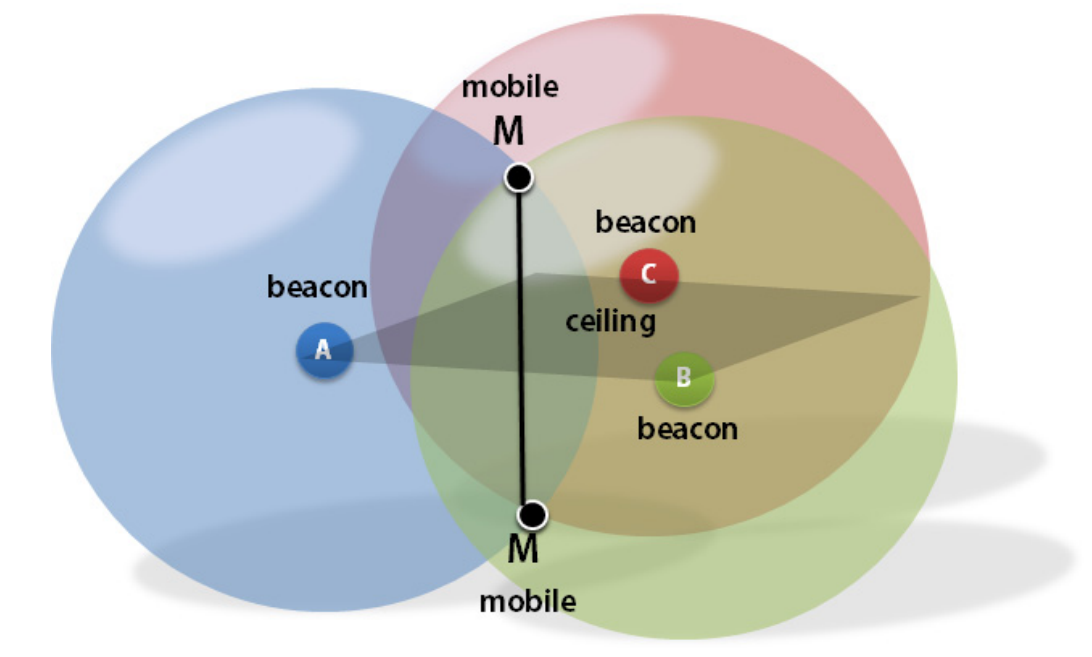
\includegraphics[width=0.62\columnwidth]{fig2.png}}
    \caption{Calculation of 3D location coordinates based on 3 sphere equations.}
    \label{fig1}
\end{figure}

\begin{figure}[htbp]
    \centerline{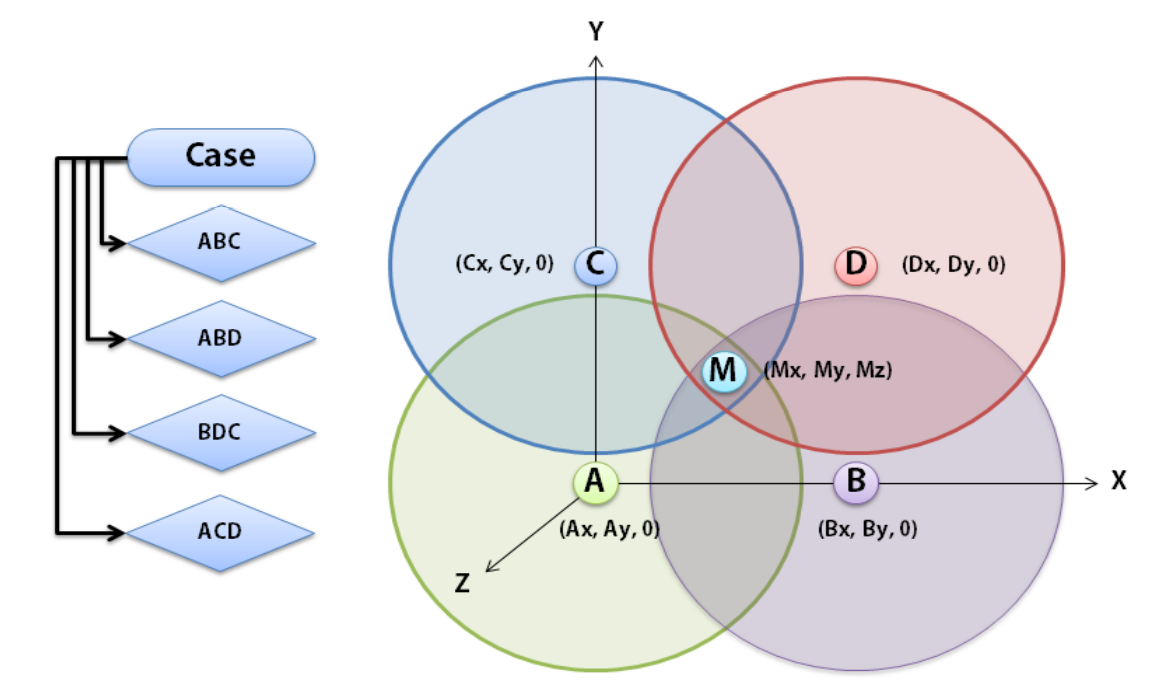
\includegraphics[width=0.62\columnwidth]{fig1.png}}
    \caption{Coordinates calculation of tag node using 4 anchor nodes.}
    \label{fig2}
\end{figure}

\subsection{Clustering method using the density of coordinates}
\textcolor{red}{Trilateration using 4 anchors gets multiple tag coordinates. However, as shown in Fig. \ref{fig1}, one of the two coordinates is far from the actual tag location. Therefore, if the clustering method using the density of coordinates proposed in this paper is used, it is possible to remove the coordinates of the tag that are far from the actual location of the tag. After that, the system can use the coordinates closest to the actual position of the tag to improve the accuracy of localization.}

\textcolor{red}{When measuring the distance between anchor and tag indoors, there is an error in the distance. For example, if a tag is tracked with 4 anchors, an obstacle between the tag and the anchor may cause errors in more than 1 of the 4 anchors. The clustering scheme proposed in this paper can quickly remove these errors.} The system finds the region with the highest density of the eight computed coordinates. First, the distance is calculated by combining two coordinates. As shown in equation \ref{eq2}, there are 28 pairs of calculated distances. \textcolor{red}{The highest density of 8 tag coordinates calculated when trilateration is performed 4 times is found by the clustering scheme.}

\begin{equation}
    \binom{8}{2} = \frac{8!}{(8-2)!2!}=28\label{eq2}
\end{equation}

As shown in Fig. \ref{fig3}, the system applies the clustering method to determine the coordinates of the tag nodes, and then selects pairs whose coordinates are within a limited range (eg, 1m). The system selects the region with the most connected nodes among the selected coordinates. Finally, one coordinate of the tag is determined by averaging the selected coordinates.

\begin{figure}[htbp]
    \centerline{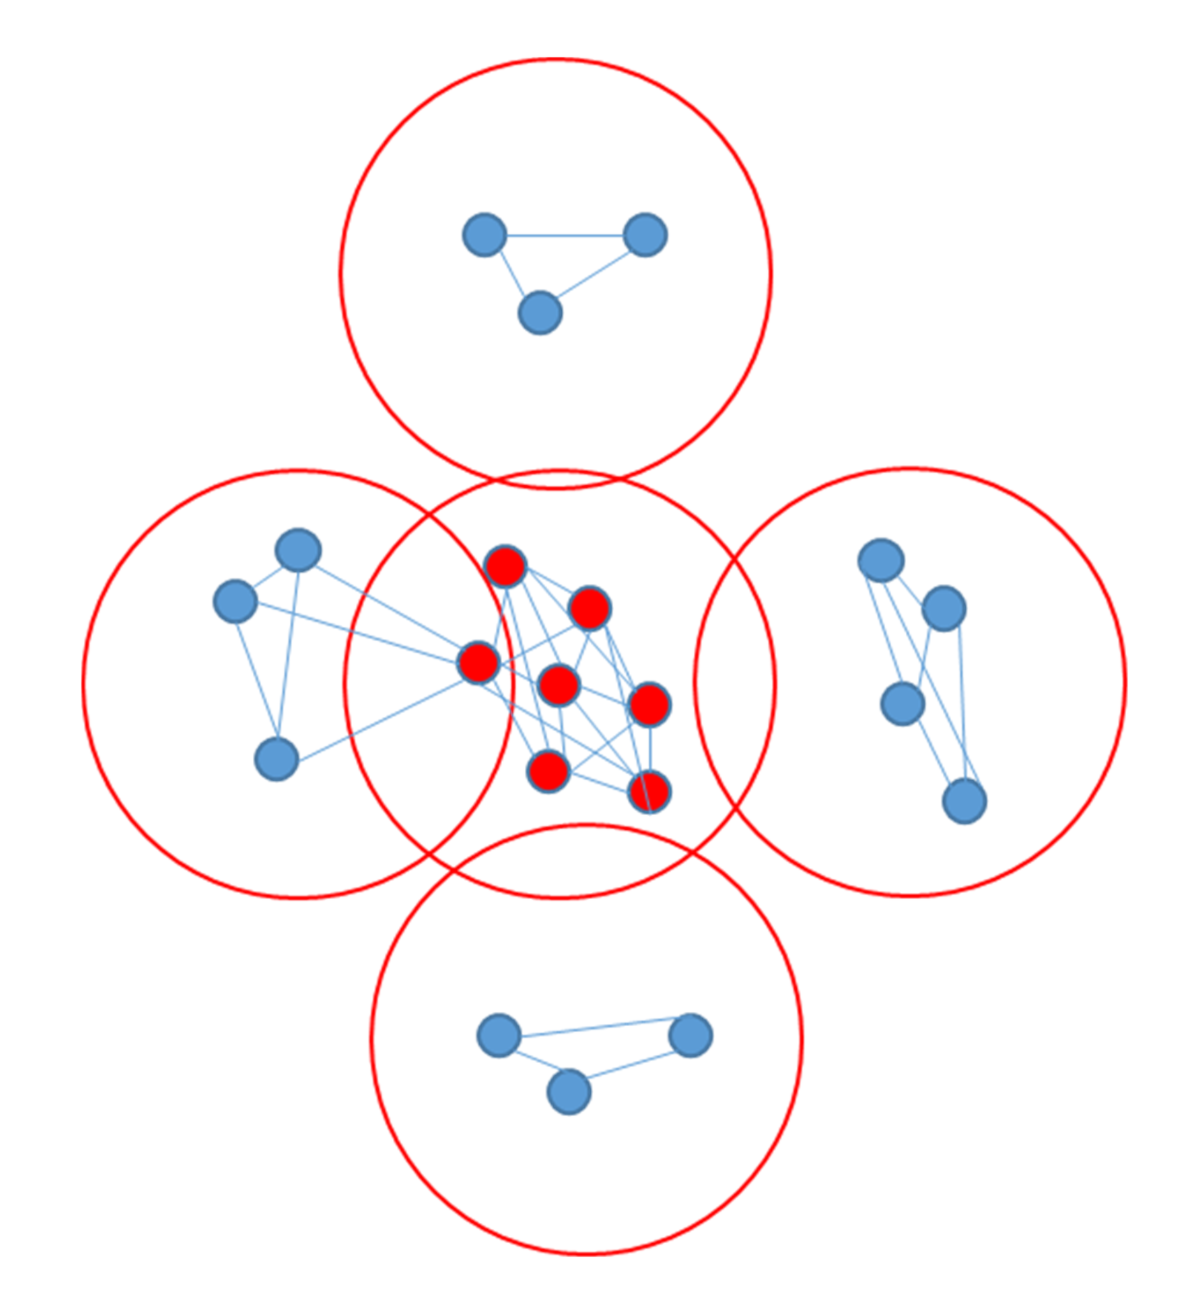
\includegraphics[width=0.62\columnwidth]{fig3.png}}
    \caption{Clustering method using the density of coordinates.}
    \label{fig3}
\end{figure}

The tag's coordinate selection fails if all the selected coordinates have the same density. In this case, as shown in Fig. \ref{fig4}, one coordinate of the tag is determined as the average of the coordinate set of the minimum distance.

\begin{figure}[htbp]
    \centerline{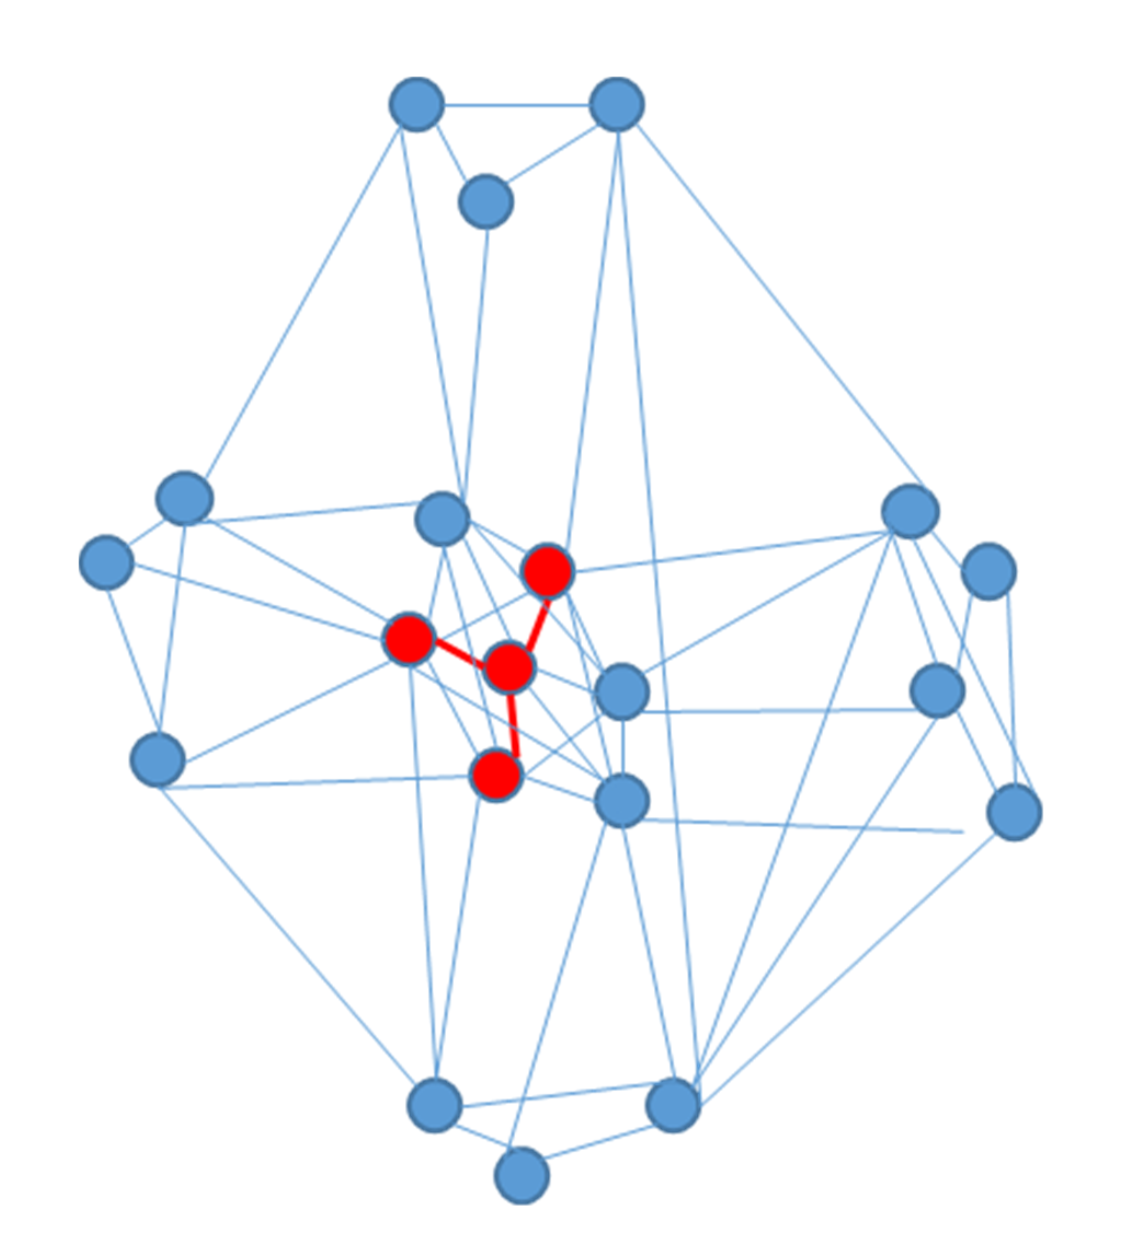
\includegraphics[width=0.62\columnwidth]{fig4.png}}
    \caption{Minimum distance method on same density of coordinates.}
    \label{fig4}
\end{figure}

\section{Experiments and Result}
\subsection{The developed localization system}

As shown in Fig. \ref{fig10}, 4 anchors, 1 tag, and 1 gateway are made to operate the real-time localization system. \textcolor{red}{The developed equipment is made of UWB wireless module. The distance between the tag and the anchor is measured using two-way ranging (TWR).}

\begin{figure}[htbp]
    \centerline{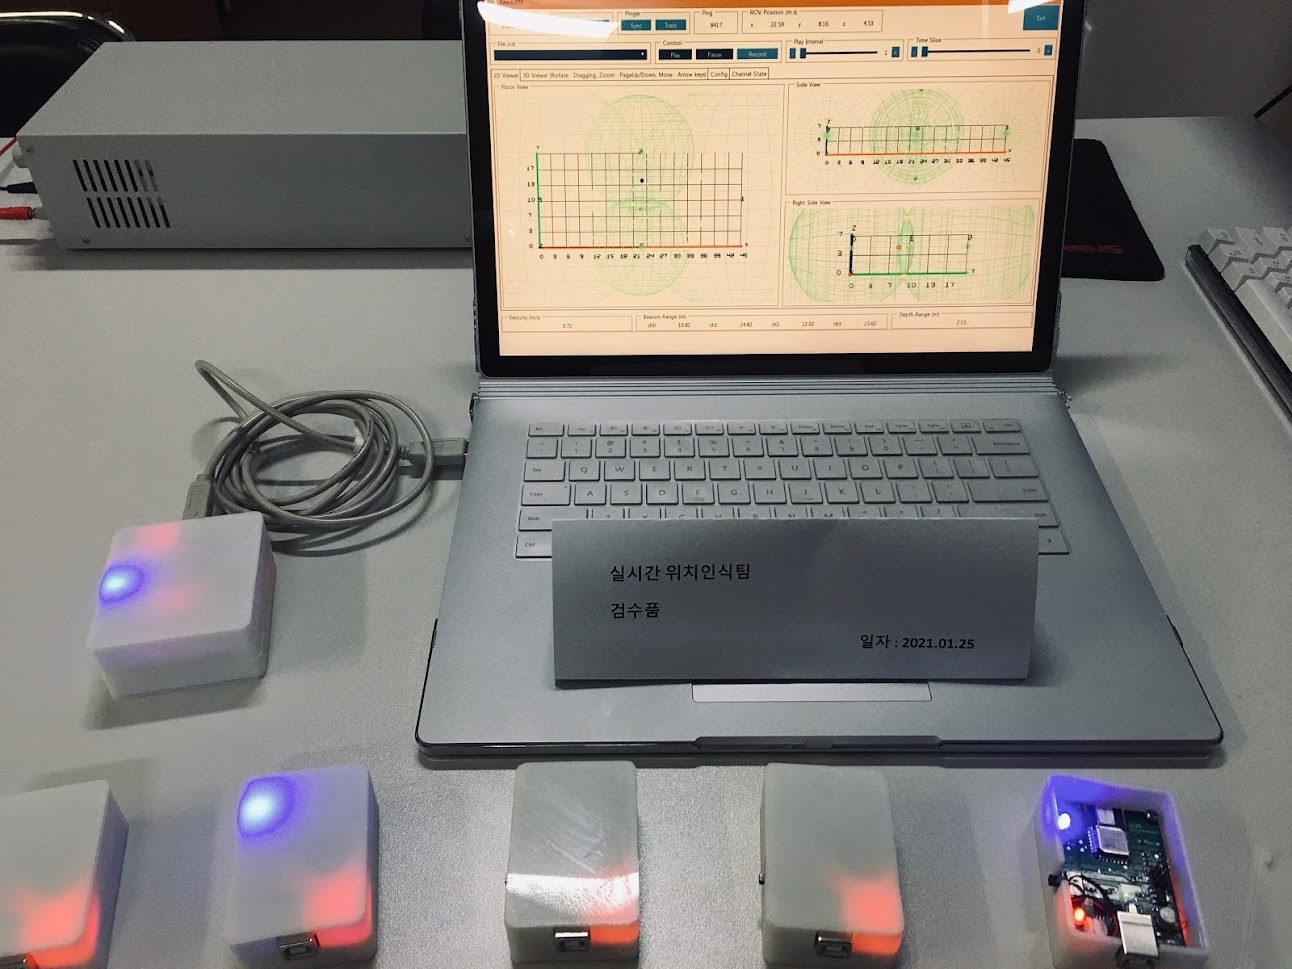
\includegraphics[width=0.62\columnwidth]{fig10.jpg}}
    \caption{Hardware for 3D localization system.}
    \label{fig10}
\end{figure}

As shown in Fig. \ref{fig5}, the developed localization scheme tracks the location of the tag when it receives a signal from the gateway. This scheme consists of top view, side view, front view and 3D image. Each screen displays the movement path of the tag in real-time. \textcolor{red}{The 3D coordinates and speed of the moving tag are displayed in time series on the graph. The system can enable or disable the proposed clustering scheme and minimum distance method. This function evaluates the performance of the proposed algorithm.}

\begin{figure}[htbp]
    \centerline{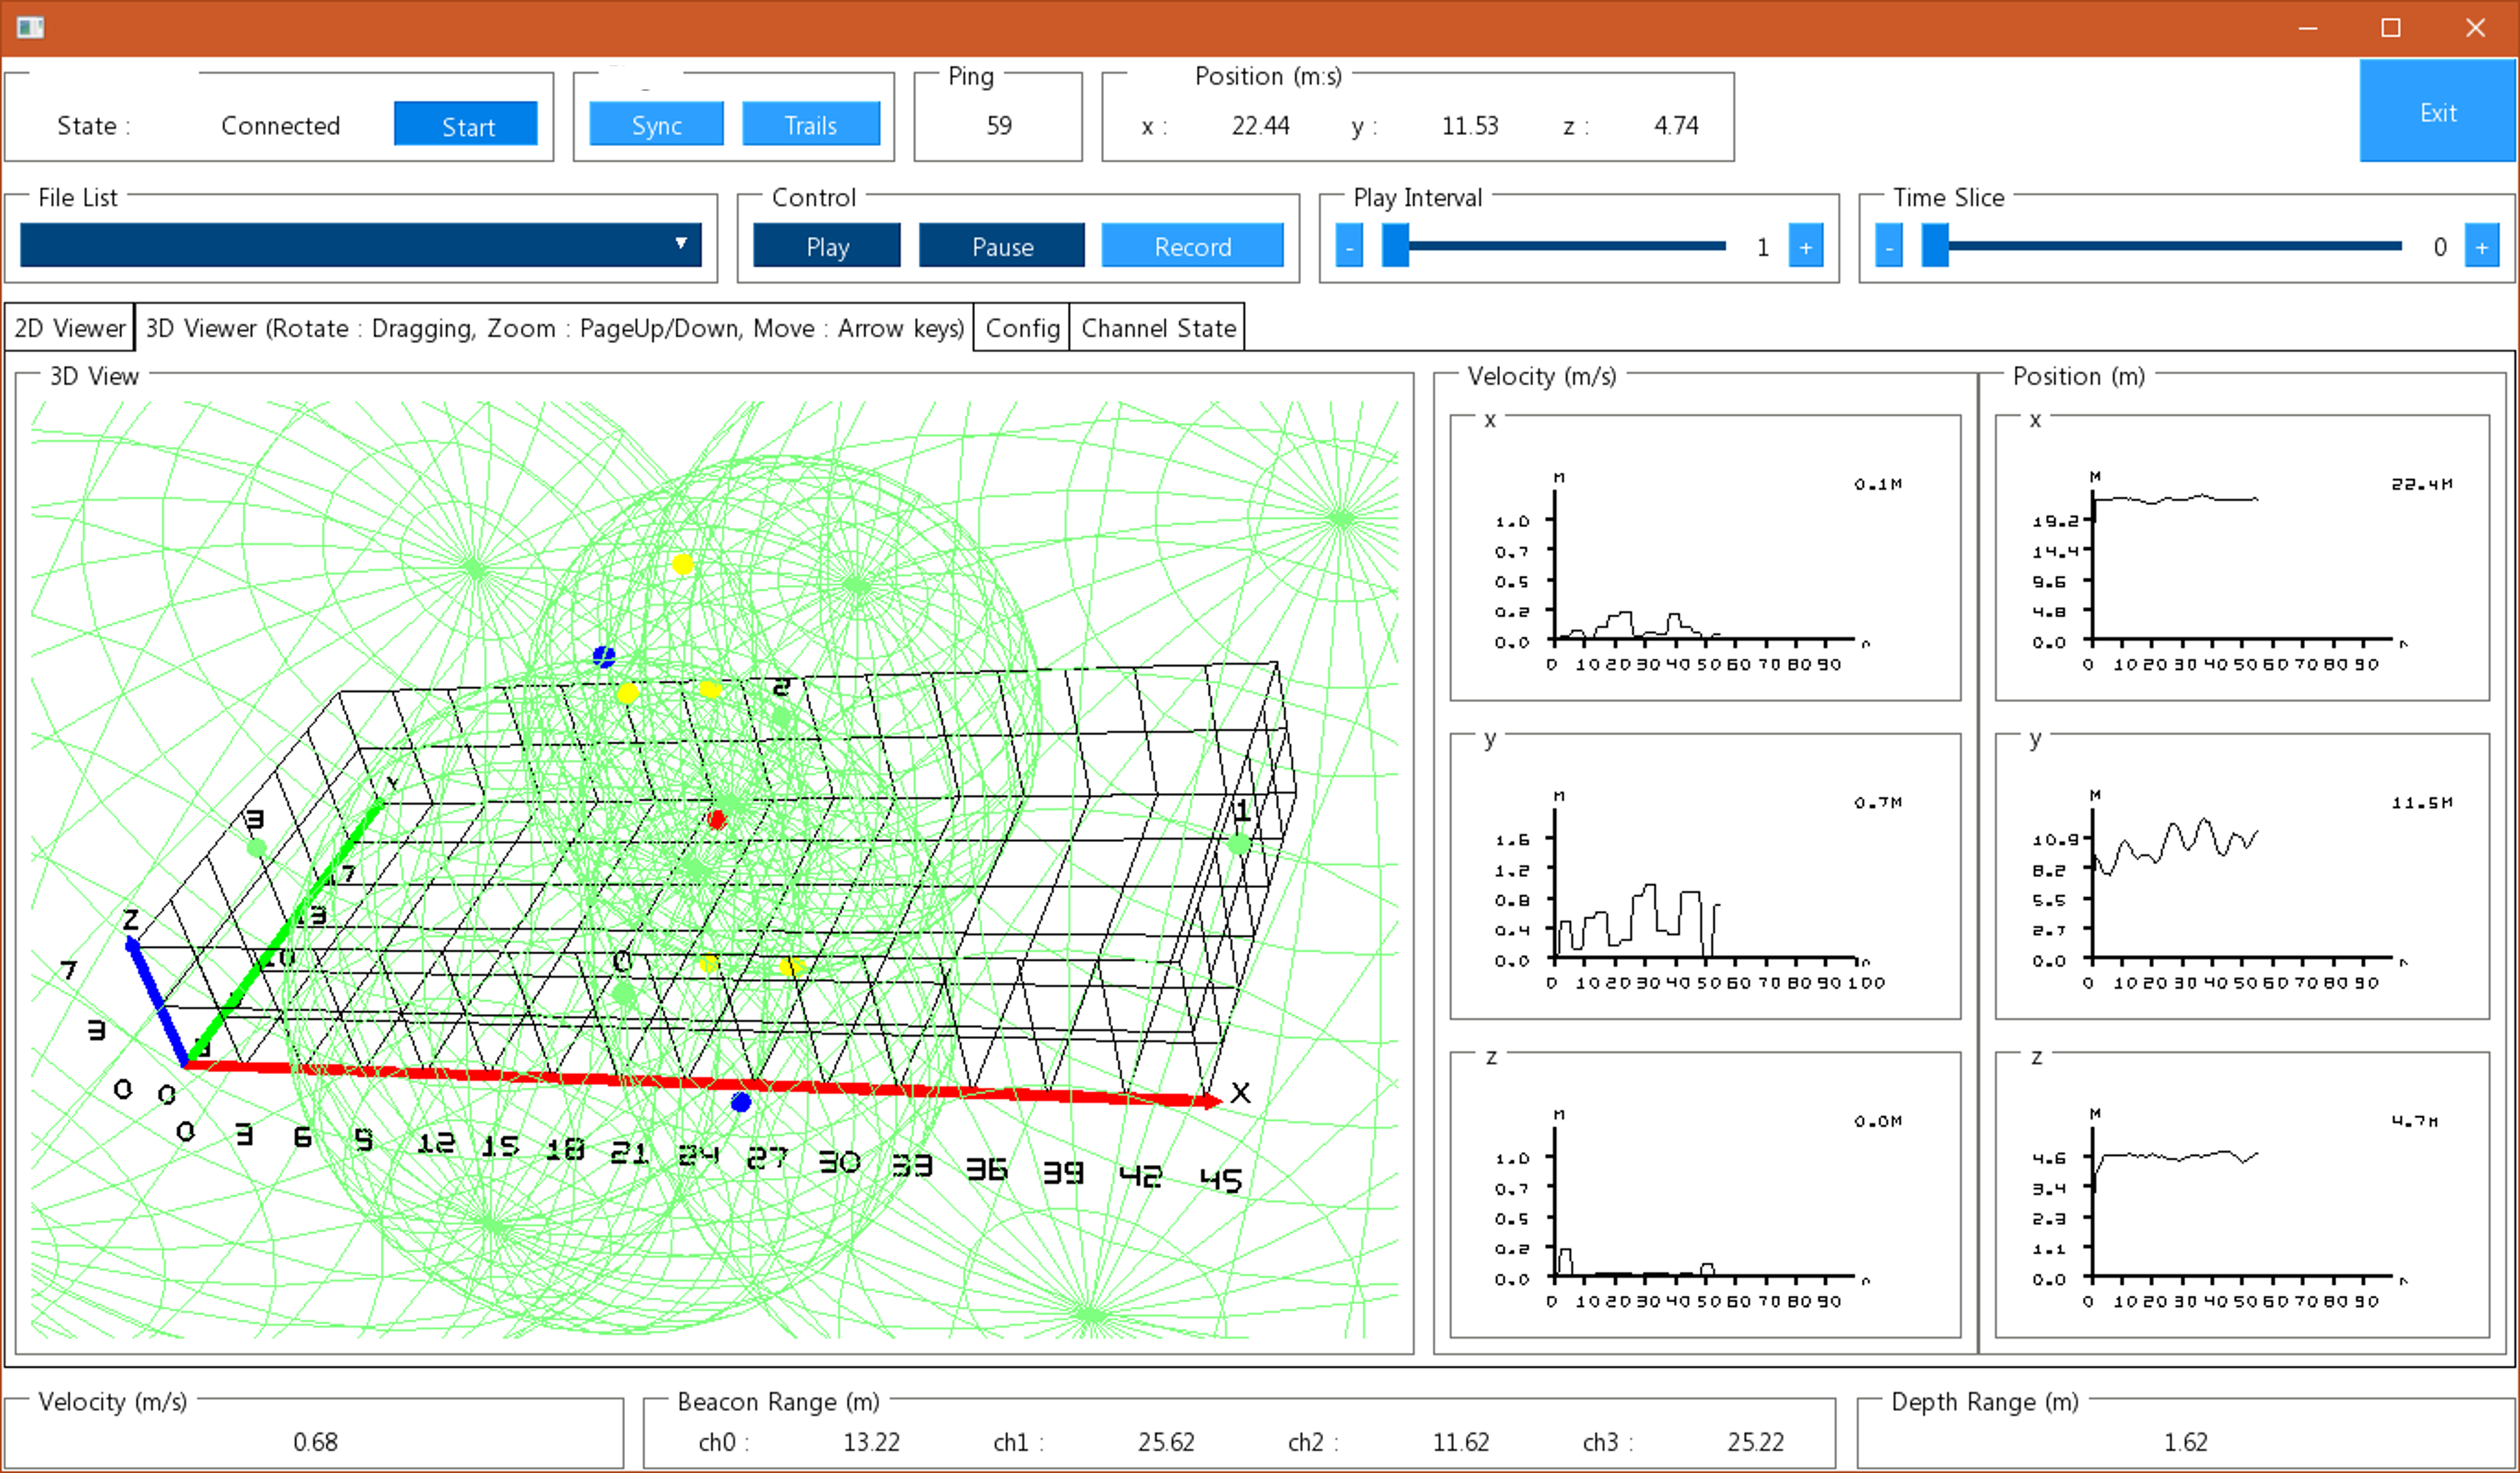
\includegraphics[width=0.62\columnwidth]{fig5.png}}
    \caption{The developed localization system.}
    \label{fig5}
\end{figure}

As shown in Fig. \ref{fig6}, the moving process of the tag is monitored in real-time in 3D space. \textcolor{red}{The x-y coordinates of the tag are shown in the top view, the y-z coordinates are shown in the side view, and the x-z coordinates are shown in the front view. The distance between the tag and the anchor is displayed as a 3D sphere. The error in the measured distance can be visually viewed using a 3D sphere.}

\begin{figure}[htbp]
    \centerline{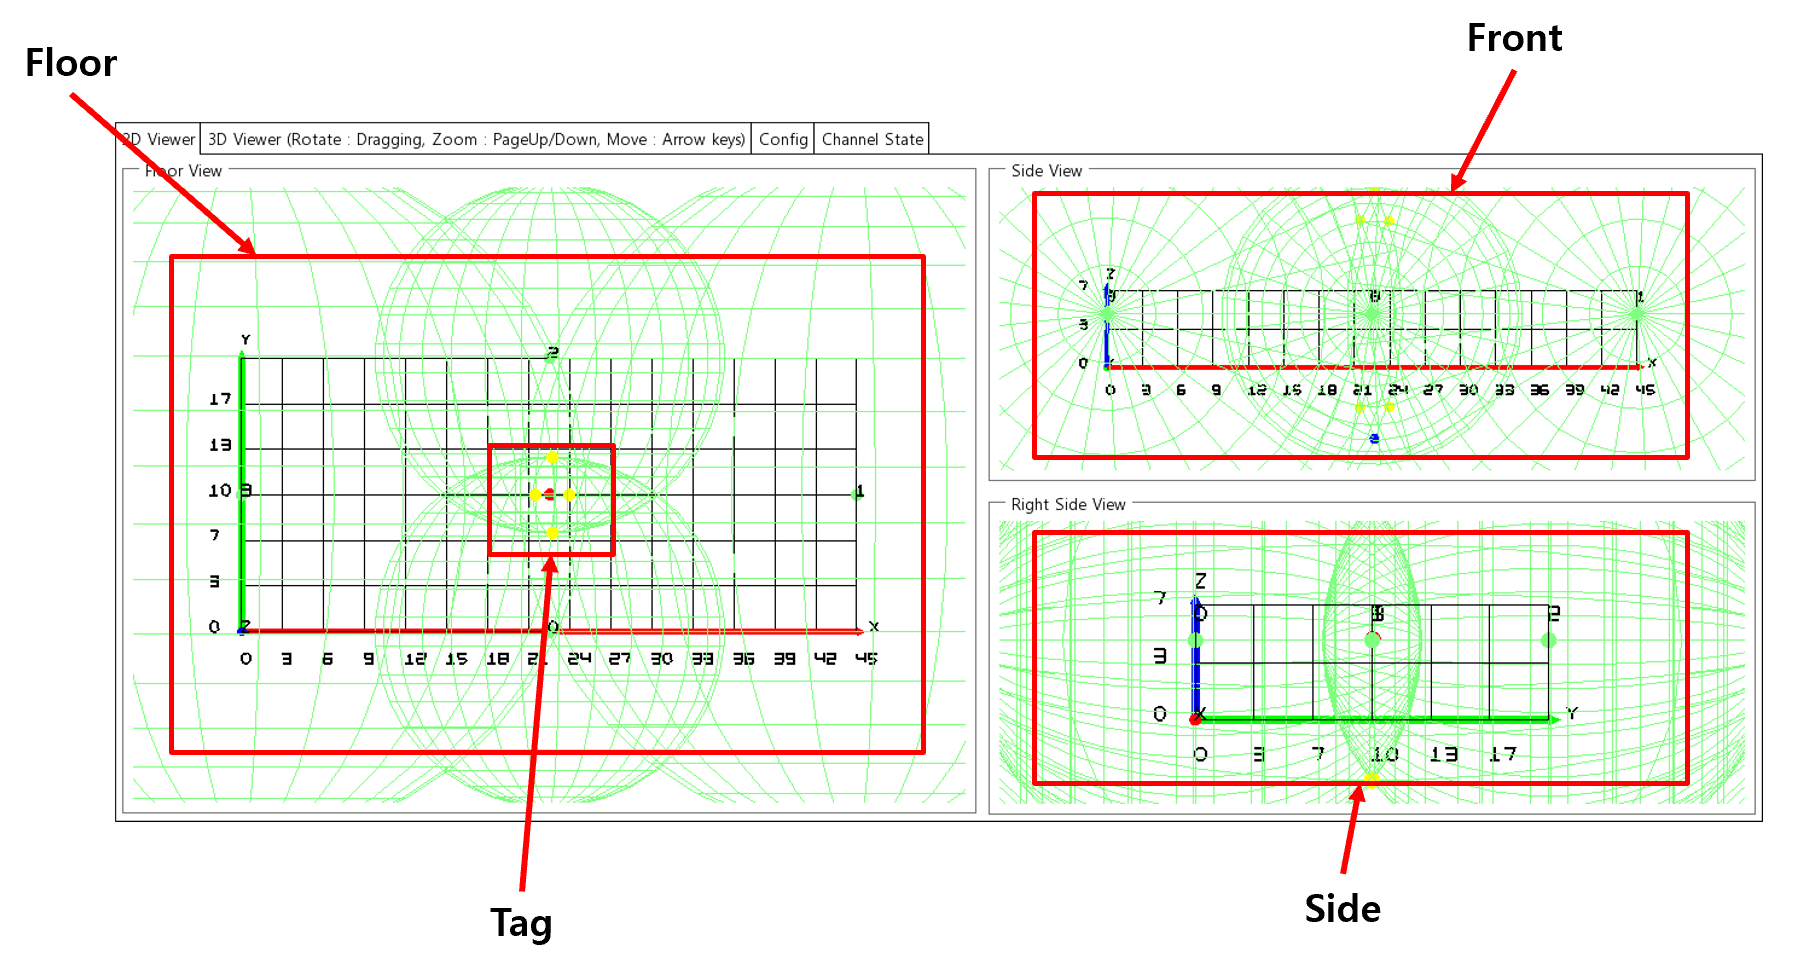
\includegraphics[width=0.62\columnwidth]{fig6.png}}
    \caption{Real time monitoring viewer.}
    \label{fig6}
\end{figure}

As shown in Fig. \ref{fig7}, the scheme shows the movement path record of the tag as a red line. \textcolor{red}{The performance of the clustering scheme can be visually evaluated using the red line of the moving path of the tag. The performance of the clustering scheme can be visually evaluated using the red line of the moving path of the tag. Real-time red lines of moving tags appear in 2D and 3D views.}

\begin{figure}[htbp]
    \centerline{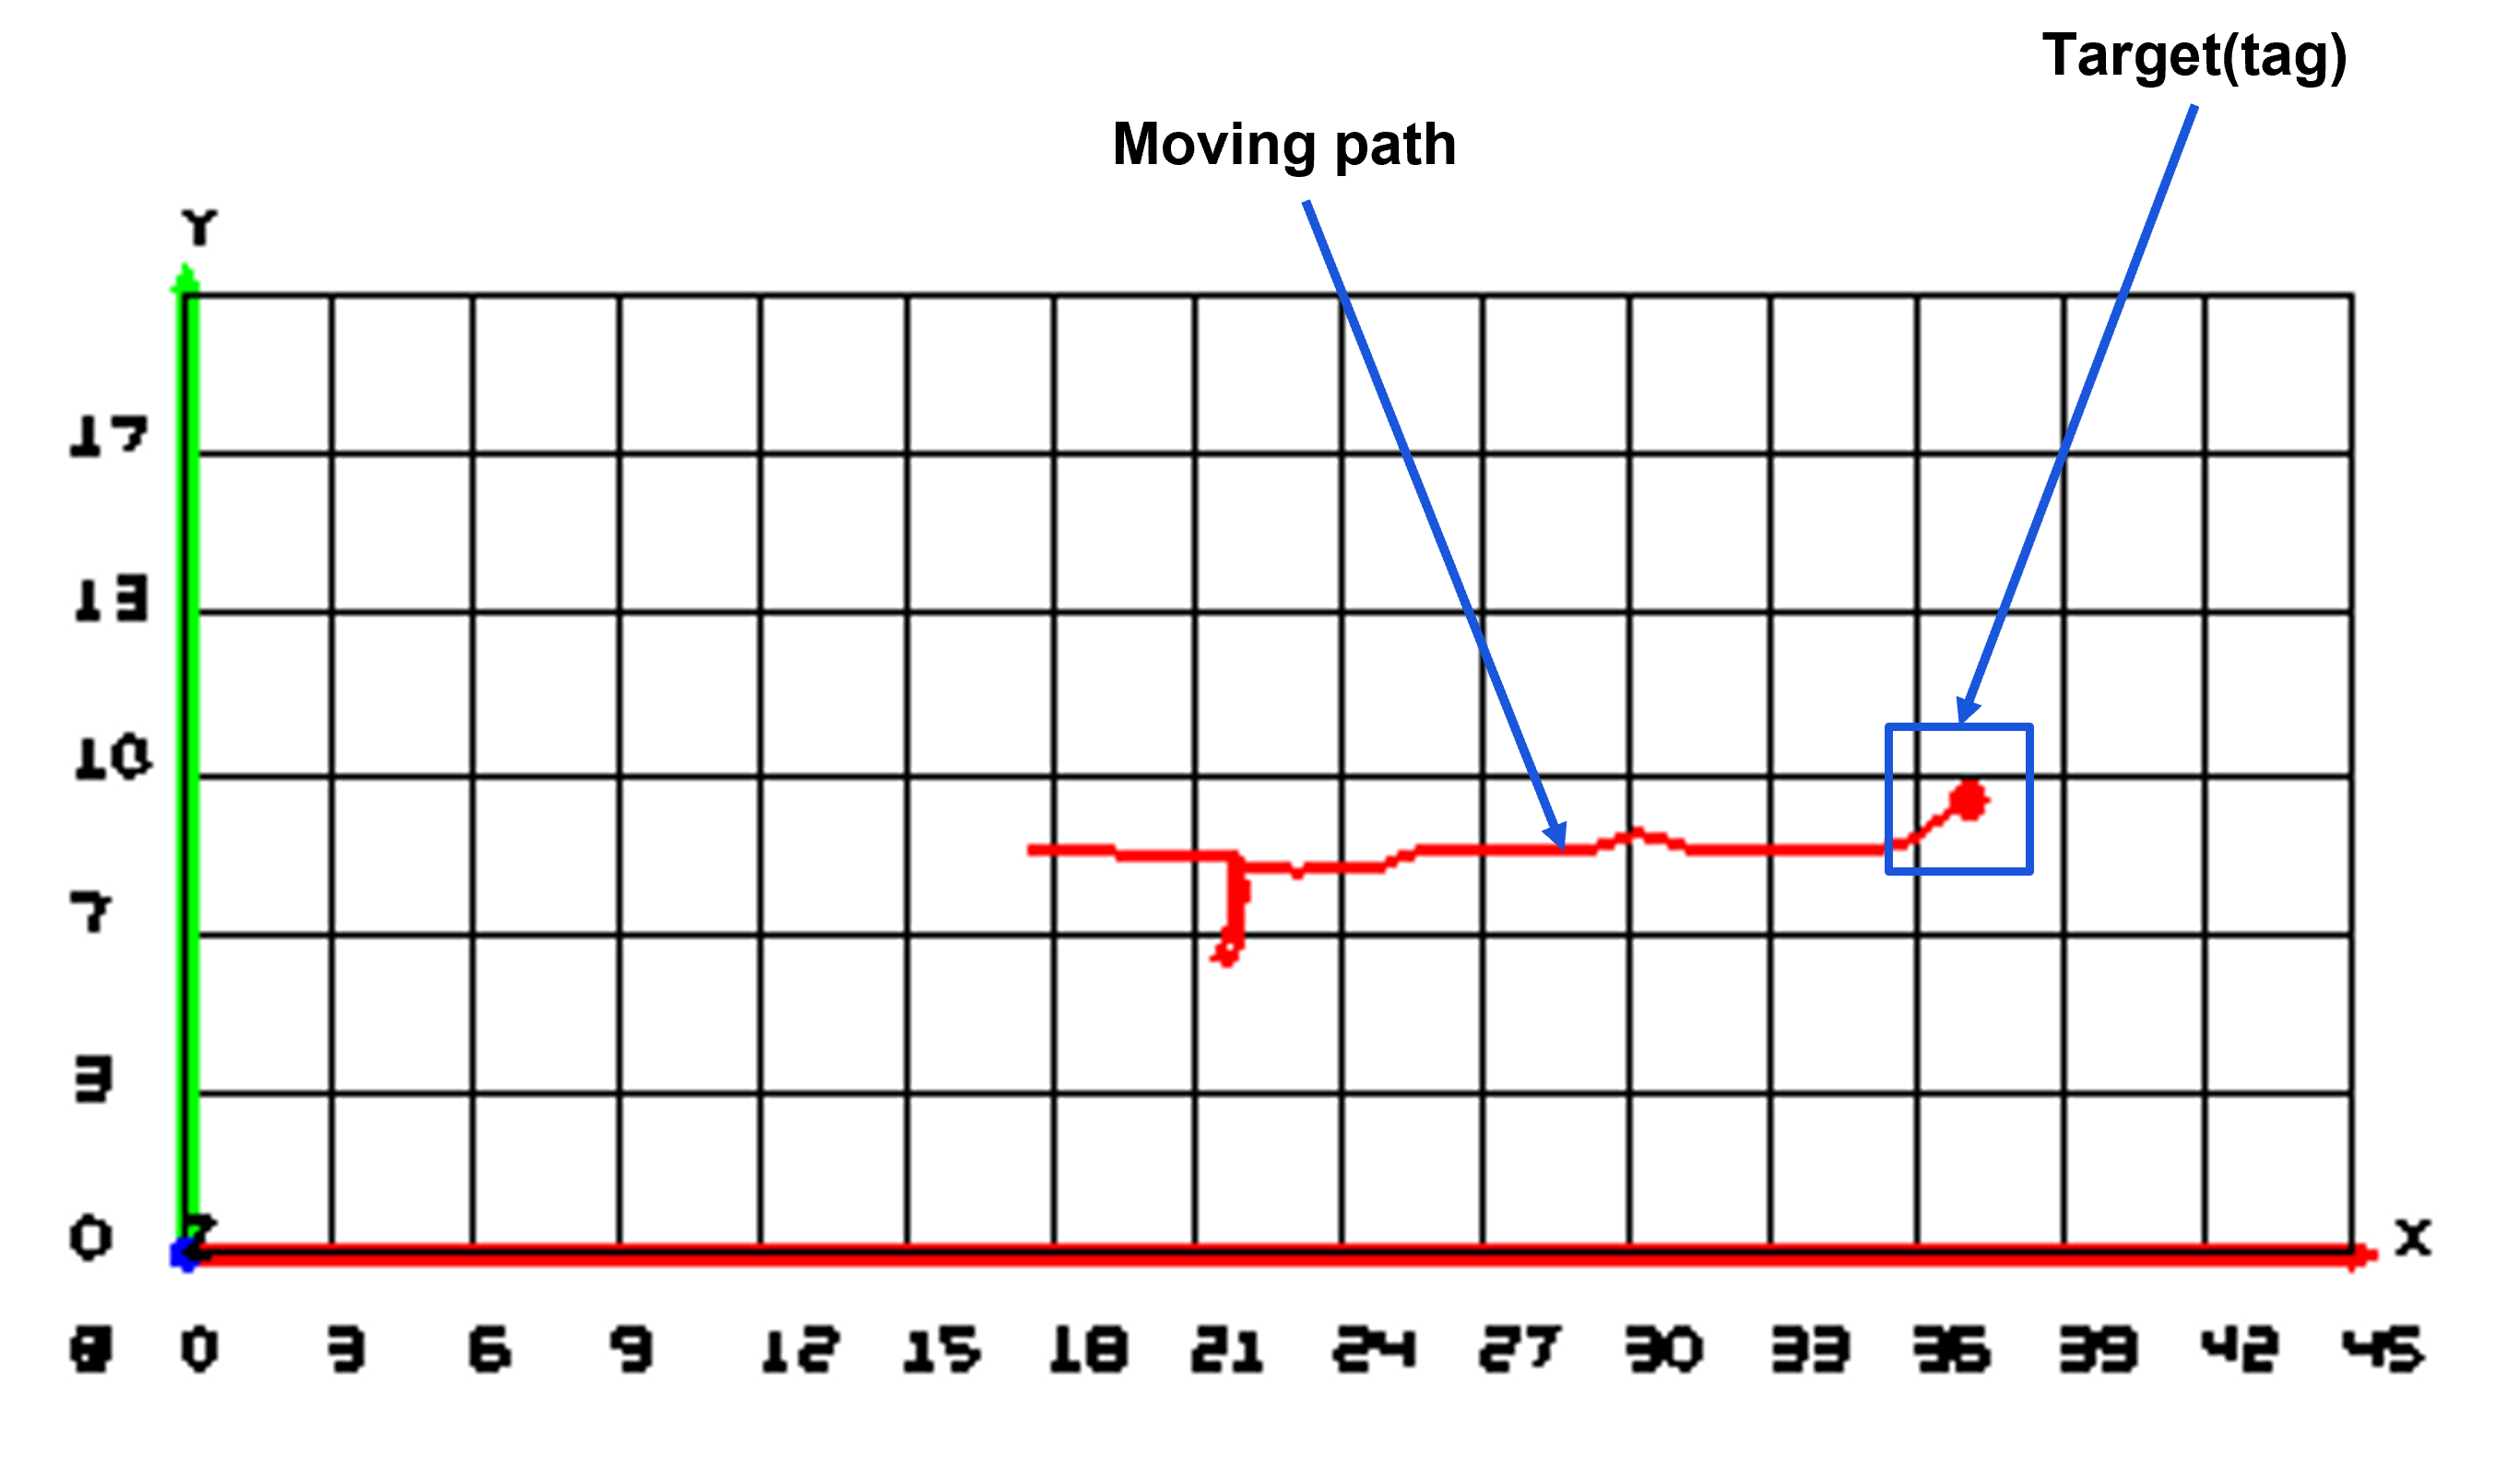
\includegraphics[width=0.62\columnwidth]{fig7.png}}
    \caption{The movement path record of the tag.}
    \label{fig7}
\end{figure}

As shown in Fig. \ref{fig8}, the scheme tracks the movement of tags in 3D space in real-time. In addition, the scheme can track the movement of the tag from various angles. \textcolor{red}{3D screen shows tag movement more intuitively than 2D screen from various angles.}

\begin{figure}[htbp]
    \centerline{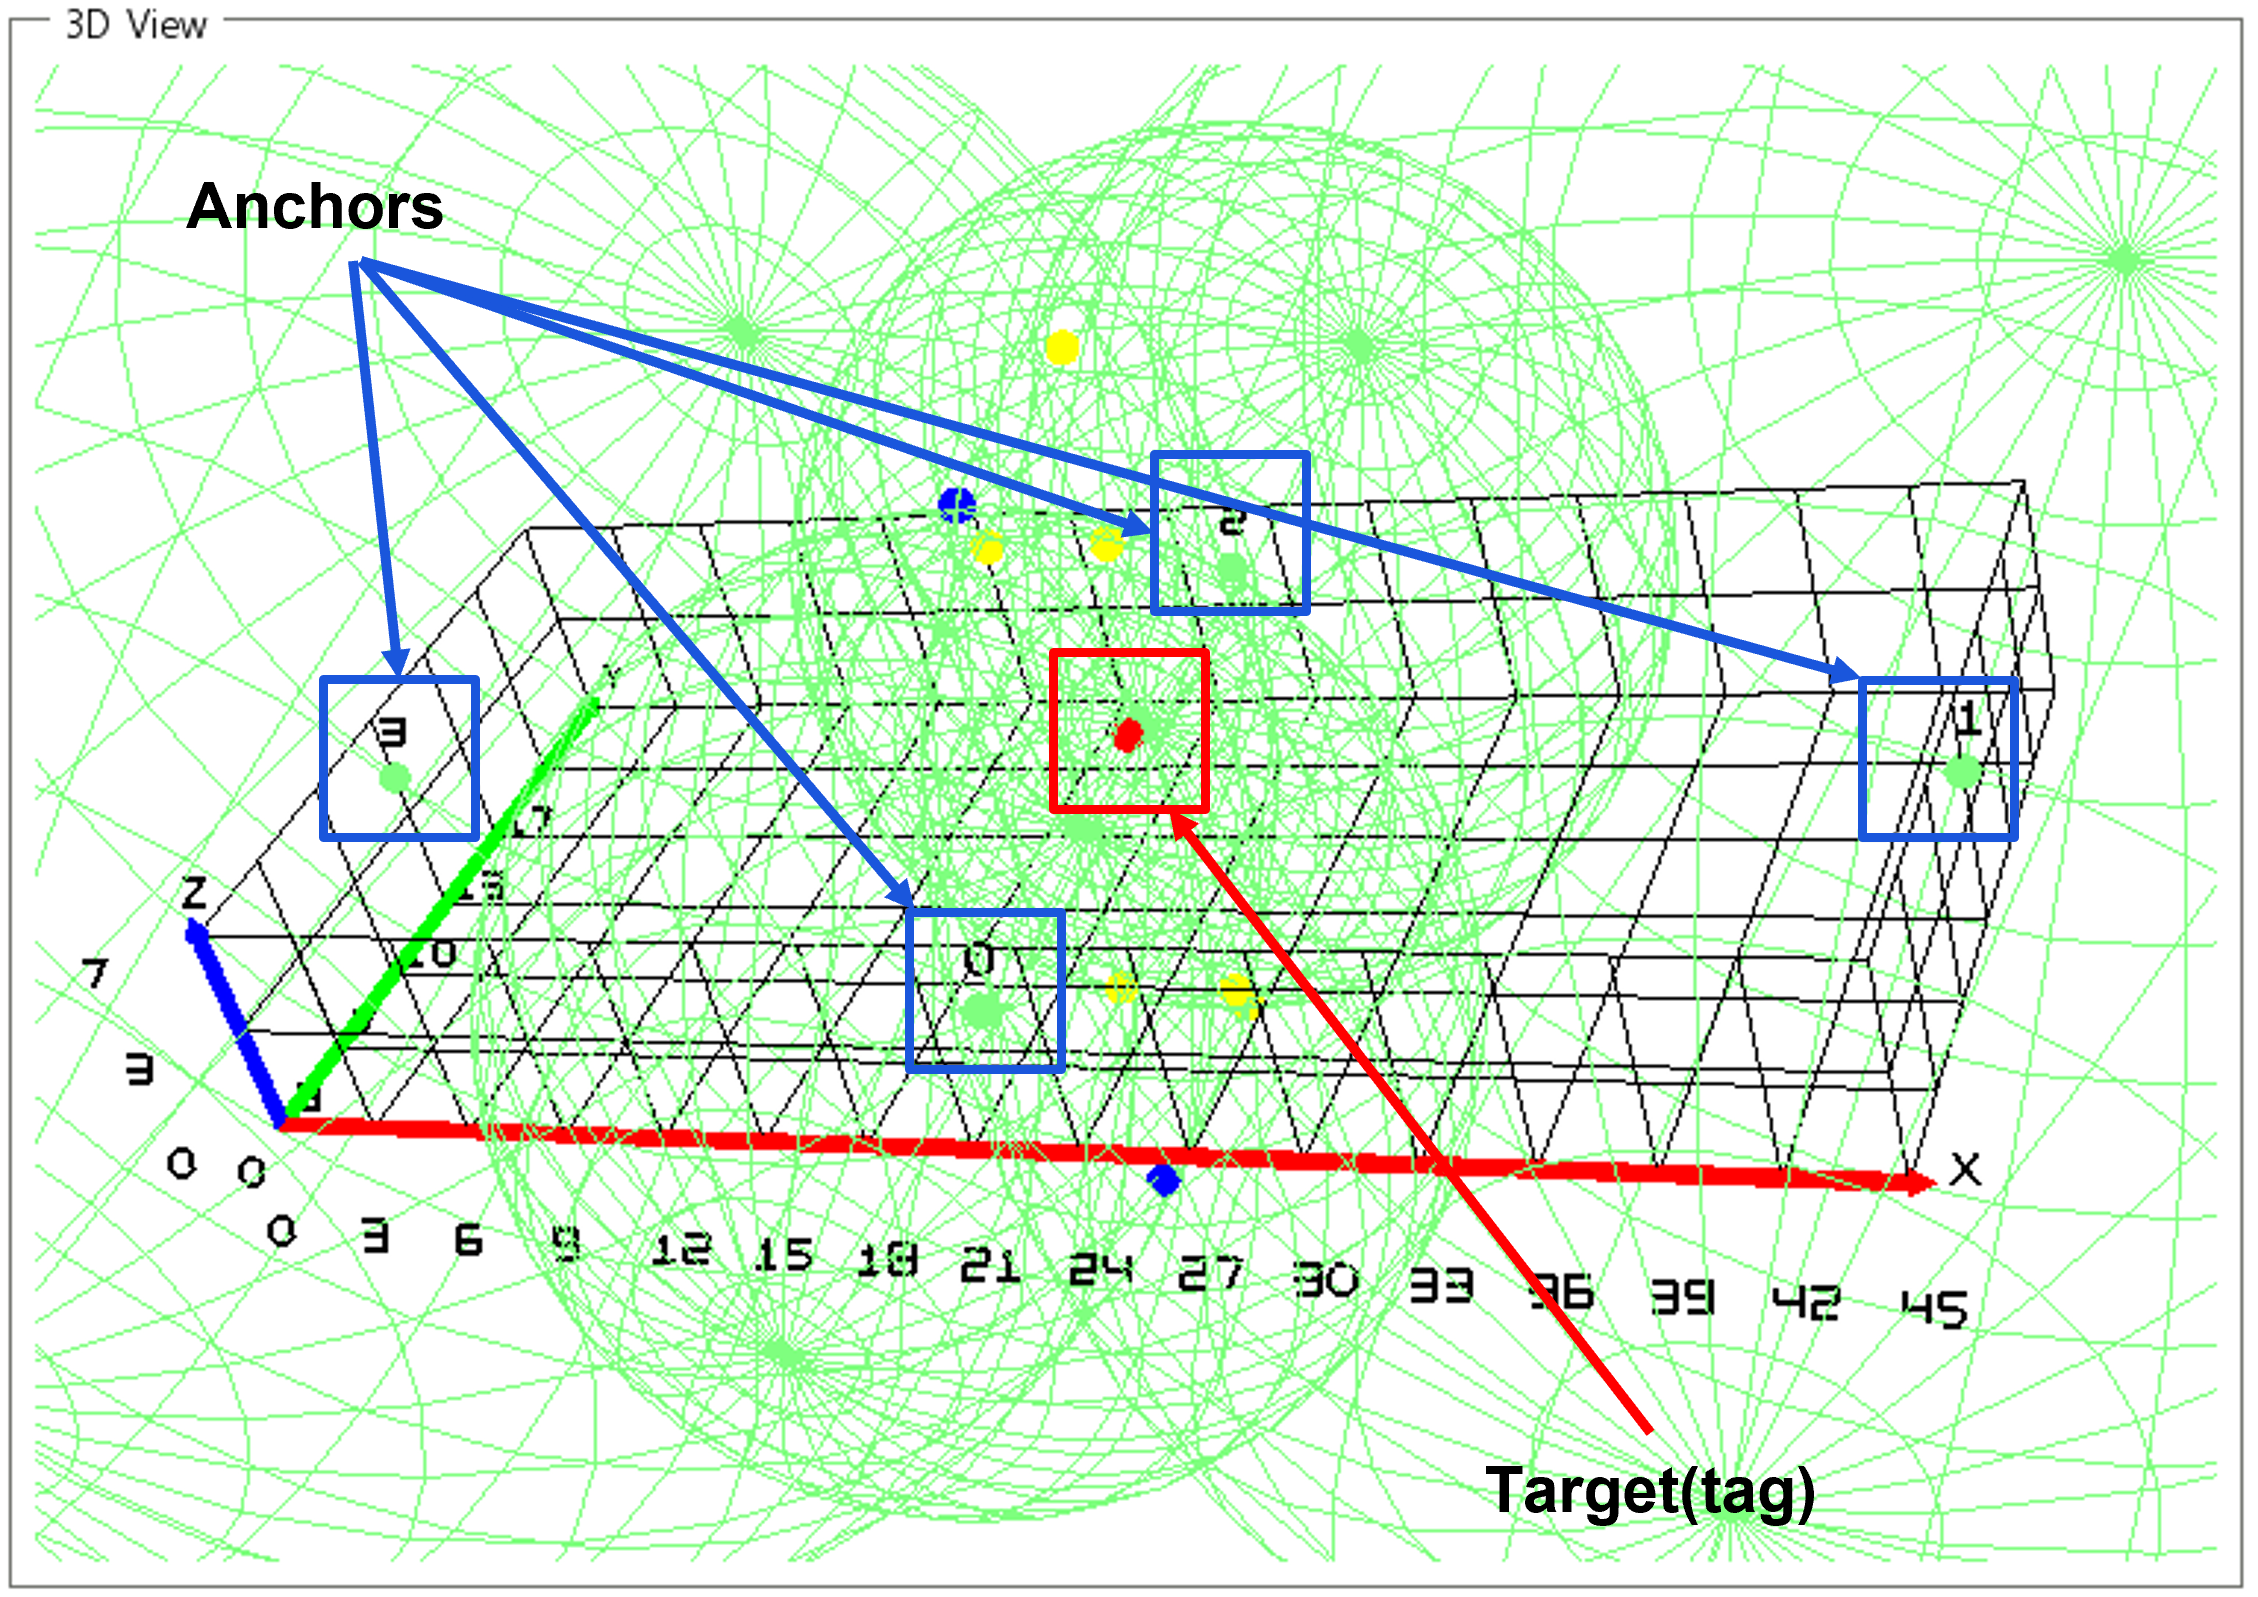
\includegraphics[width=0.62\columnwidth]{fig8.png}}
    \caption{3D localization from various angles.}
    \label{fig8}
\end{figure}

As shown in Fig. \ref{fig9}, the tag's speed and position are displayed as graphs on each coordinate axis and are updated in real-time. \textcolor{red}{The performance of the proposed clustering scheme can be visually evaluated using these graphs.}

\begin{figure}[htbp]
    \centerline{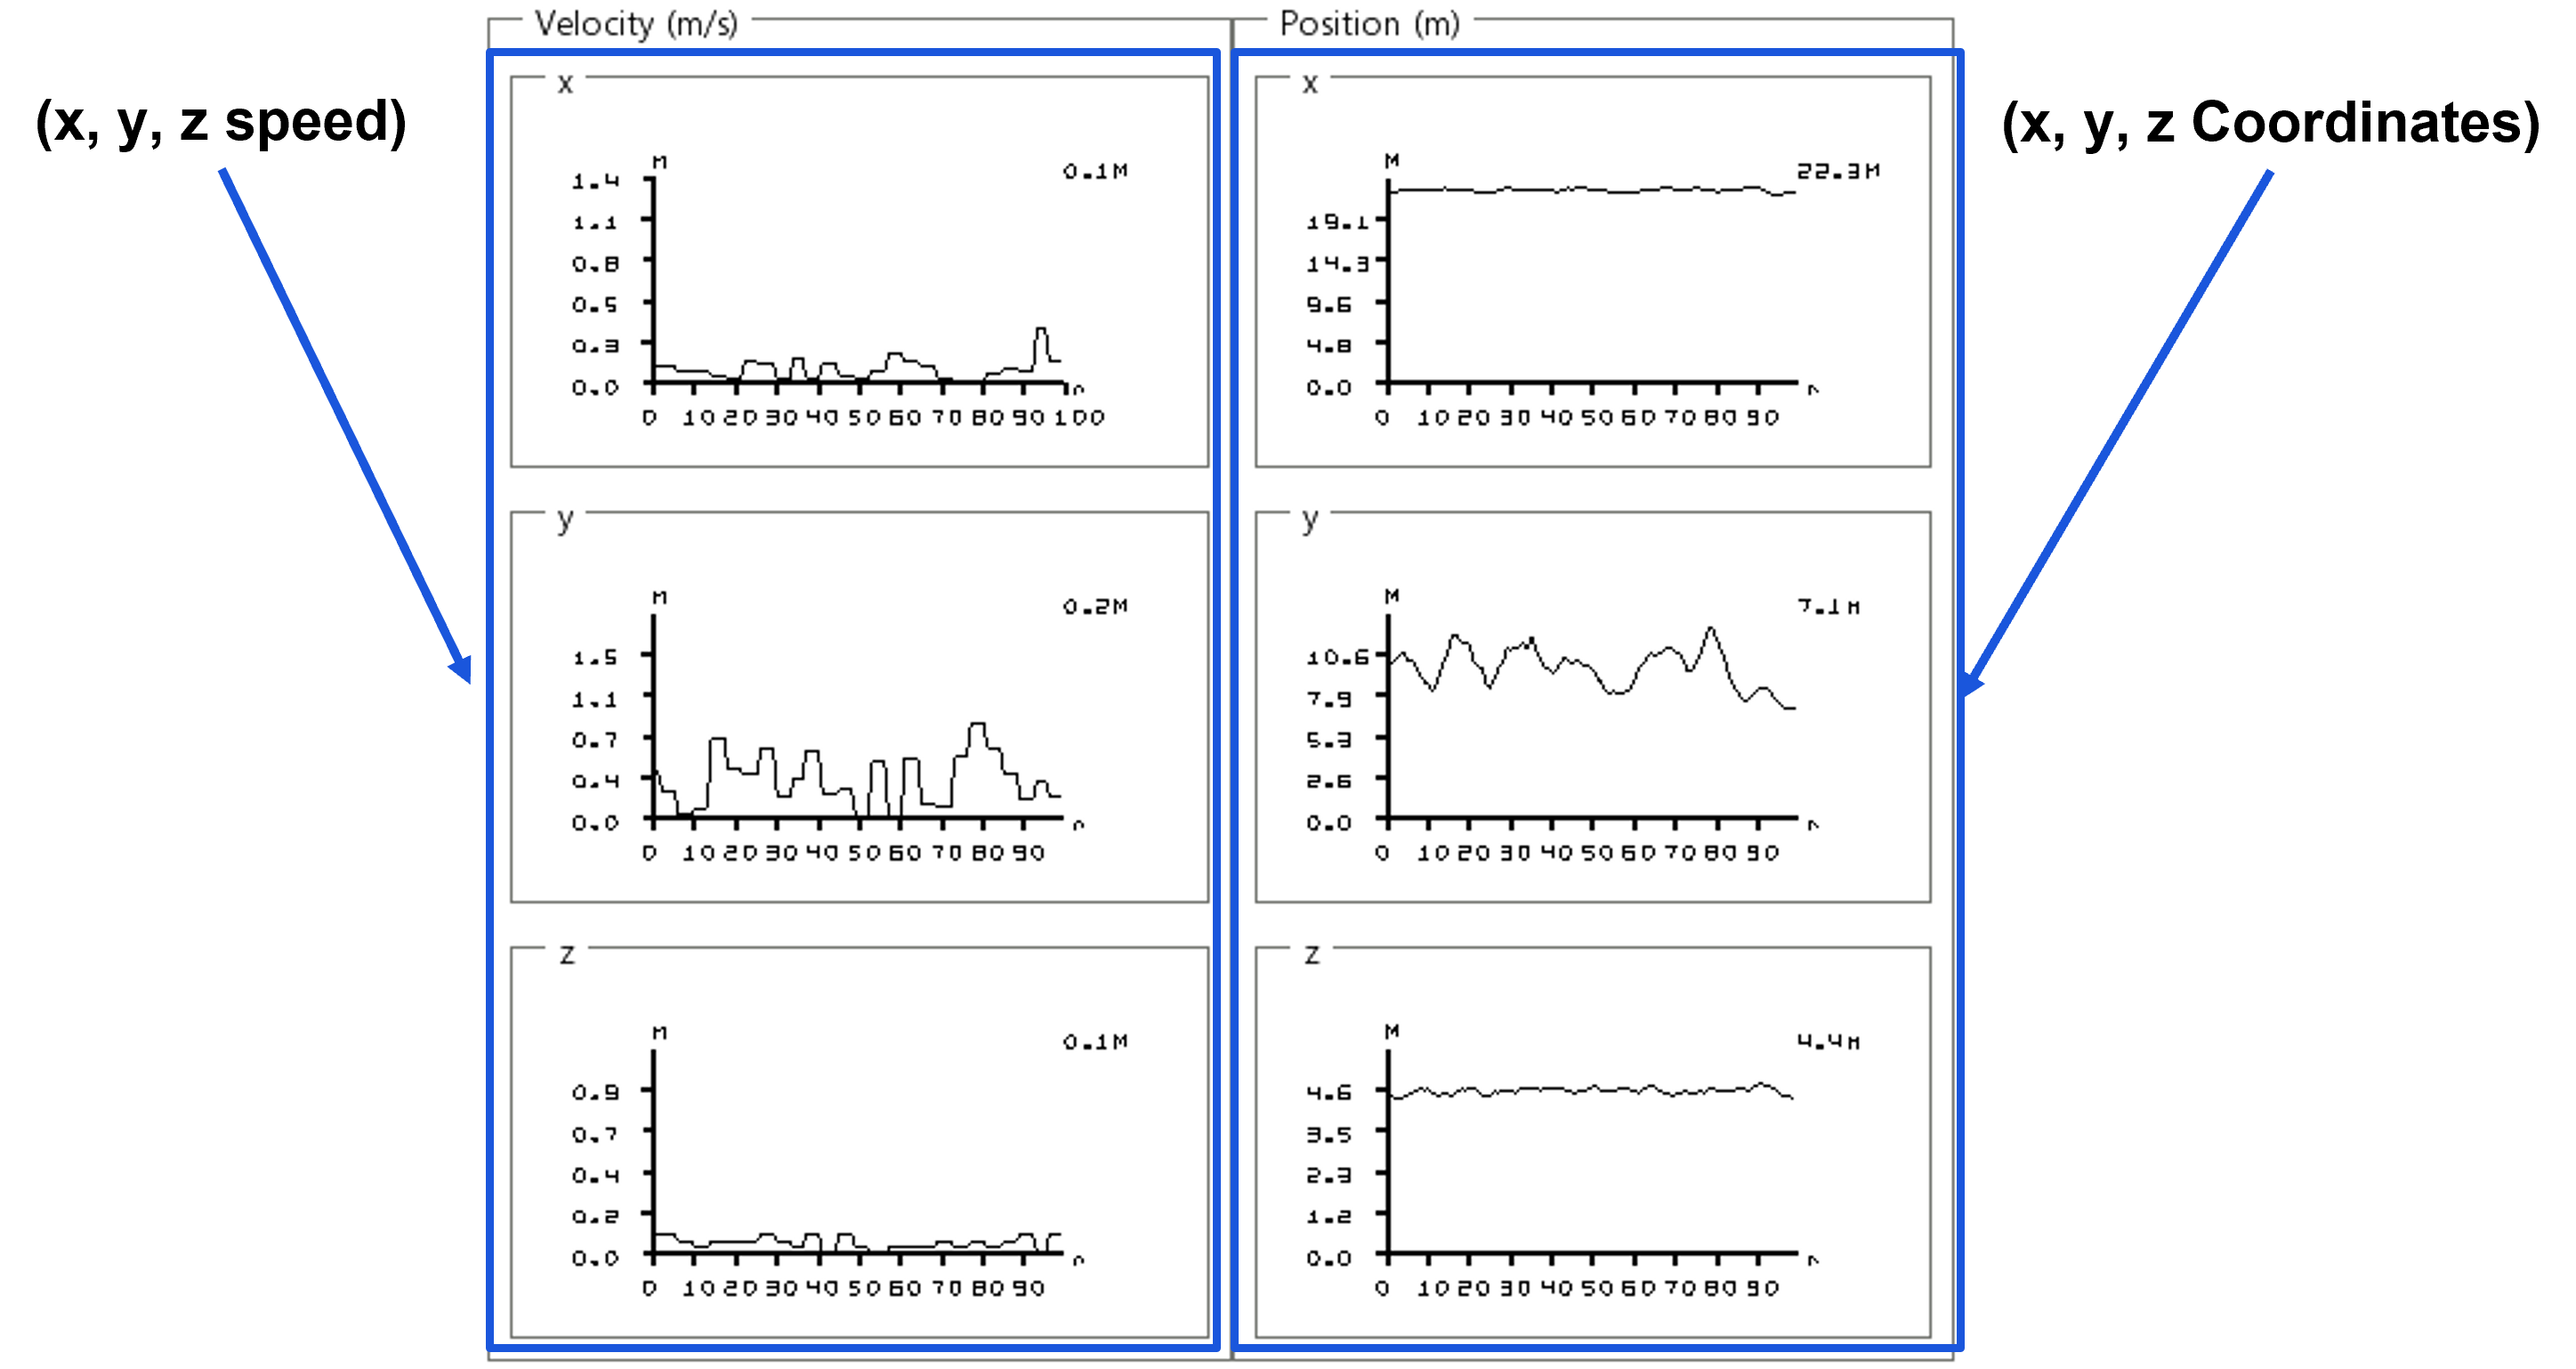
\includegraphics[width=0.62\columnwidth]{fig9.png}}
    \caption{Real-time speed and position graphs of tags.}
    \label{fig9}
\end{figure}

\subsection{\textcolor{red}{Experimentation Results}}
The performance evaluation of the localization method is divided into the case where there is no method, only the clustering method is applied, or the clustering method is combined with the minimum distance method. As shown in Table \ref{tab1}, the experiment combining the clustering method and the minimum distance method has the smallest standard error.

\begin{table}[htbp]
    \caption{Performance results of localization scheme.}
    \begin{center}
        \begin{tabular}{|c|c|c|c|}
            \hline
            \textbf{Measurement} & \multicolumn{3}{|c|}{\textbf{Standard error of method}}                                                                       \\
            \cline{2-4}
            \textbf{Unit}        & \textbf{\textit{None}}                                  & \textbf{\textit{Clustering}} & \textbf{\textit{+ Minimum distance}} \\
            \hline
            cm                   & 46.3                                                    & 12.7                         & 10.2                                 \\
            \hline
        \end{tabular}
        \label{tab1}
    \end{center}
\end{table}

\section{Conclusion}

In this paper, a real-time clustering scheme is proposed to improve the localization performance of a 3D localization system using a wireless sensor. In addition, the hardware and software were actually developed to evaluate the performance of the proposed scheme. It was confirmed that the standard error of the measured tag coordinates decreased in the performance evaluation. In the future, based on this study, we plan to evaluate the performance of the proposed scheme in a multi-tag environment.

\section*{Acknowledgment}

This research was supported by the BB21plus funded by Busan Metropolitan City and Busan Institute for Talent \& Lifelong Education (BIT).
This work was supported by the National Research Foundation of Korea (NRF) grant funded by the Korea government (MSIT) (No. 2019R1F1A1062670).

\begin{thebibliography}{00}
    \bibitem{b1} Park, Jee Woong, Cho, Yong K., Martinez, Diego, "A BIM and UWB integrated Mobile Robot Navigation System for Indoor Position Tracking Applications," 6(2), pp.30-39, 2016.
    \bibitem{b2} J. Maneesilp, C. Wang, H. Wu and N. Tzeng, "RFID Support for Accurate 3D Localization," in IEEE Transactions on Computers, vol. 62, no. 7, doi: 10.1109/TC.2012.83, pp.1447-1459, July 2013.
    \bibitem{b3} M. Yoon, M. Kim and C. Lee, "A Dynamic Cell Clustering Algorithm for Maximization of Coordination Gain in Uplink Coordinated System," in IEEE Transactions on Vehicular Technology, vol. 65, no. 3, doi: 10.1109/TVT.2015.2413899, pp.1752-1760, March 2016.
    \textcolor{red}{
    \bibitem{b4} Y. K. Cho and J. Youn, “Wireless Sensor-driven Intelligent Navigation Robots for Indoor Construction Site Security and Safety,” in 23rd ISARC, pp.493–498, 2006.
    \bibitem{b5} J. Park, Y. K. Cho, and C. Ahn, “Wireless Tracking System Integrated with BIM for Indoor Construction Applications,” in Proceedings of The 2016 Construction Research Congress (CRC), 2016.
    \bibitem{b6} F. Subhan, H. Hasbullah, and K. Ashraf, "Kalman filter-based hybrid indoor position estimation technique in bluetooth networks," Int. J. Navig. Obs. 2013.
    \bibitem{b7} K. Kim and Y. Cho, "BIM-Based Planning of Temporary Structures for Construction Safety," Comput. Civ. Eng. 2015.
    \bibitem{b8} X. Guo, Z. Chen, X. Hu and X. Li, "Multi-Source Localization Using Time of Arrival Self-Clustering Method in Wireless Sensor Networks," in IEEE Access, vol. 7, pp. 82110-82121, 2019.
    }
\end{thebibliography}

\end{document}
